%! TEX root = /home/hsartoris/sproj/writeup/main.tex
\graphicspath{ {resources/models/3neurEx/} {resources/models/3neurEx/weights/} } 

\chapter{Results}
\label{results}
\section{3-neuron generator}
\label{results_3neur}
We first consider a generator network consisting of three nodes connected as in 
figure \ref{fig:2simplex+adjacency}. All weights are binary, and a spike rate of 
.25 was used.\footnote{SEE APPENDIX	for information on spike rates}

\begin{table}[h]
	\centering
	
\begin{tikzpicture}[baseline=(current bounding box.center),->,>=stealth', 
	node distance=5em, semithick]
	\tikzstyle{every state}=[fill=none, draw=black, text=black]

	\node[state] (0) {0};
	\node[state] (1) [right of=0] {1};
	\node[state] (2) [below right of=0] {2};

	\path 	(0) edge node {} (1)
			(0) edge node {} (2)
			(1) edge node {} (2);
\end{tikzpicture}

	\hspace{2em}
	\begin{tabular}{l|lll}
		  & 0 & 1 & 2\\
		\hline
		0 & 0 & 0 & 0\\
		1 & 1 & 0 & 0\\
		2 & 1 & 1 & 0
	\end{tabular}
	\captionof{figure}{Network structure and adjacency matrix of the generator.  
	(Reproduced from Figure \ref{fig:toyex})}
	\label{fig:2simplex+adjacency}
\end{table}\noindent
While reconstructing a graph comprising only three nodes is not much of a feat, 
this simplified case allows us to demonstrate that our convolutional approach is 
capable of reconstruction at all. Furthermore, the small network size requires 
few timesteps and a small interlayer featurespace; i.e., $b,d<10$. This results 
in a relatively simple set of transitions, allowing us to explore and understand 
the inner workings of the network.

\subsection{Example Model}
\label{subsec:3neurex}
The following data are pulled from a model trained on data produced by the 
generator in figure \ref{fig:2simplex+adjacency}. Figure 
\ref{fig:3neur_loss+params} demonstrates the model's loss over time. In this 
example, \textit{b} and \textit{d} were pushed down in order to allow for better 
comprehension of the internal mechanics; the loss tends to converge more 
effectively and evenly given more computation power.
\begin{table}[ht]
	\centering
	\begin{minipage}{.48\textwidth}
	\resizebox{\textwidth}{!}{
		\begin{tikzpicture}
			\begin{semilogyaxis} [xlabel=Step, ylabel=Loss, scaled x 
				ticks=false,
				axis lines*=left,
				xtick={1,3750,7500,11250,15000},
				extra y ticks={.05,.5}, extra y tick style={grid=major},
%				ytick={0,.1,.5,1}, 
				yticklabel style={	/pgf/number format/precision=2,
									/pgf/number format/fixed}]
				\addplot [color=black] table [x=Step, y=Loss, col sep=comma, 
			mark=none, smooth] {../resources/models/3neurEx/losses};
			\end{semilogyaxis}
		\end{tikzpicture}
	}
	\end{minipage}
	\hfill
	\begin{minipage}{.48\textwidth}
		\centering
		\begin{tabular}{lr}
			b (timesteps) & 8\\
			d& 5\\
			Batch size& 32\\
			Learning rate& .0005\\
			Training samples& 17984\\
			Validation samples& 4512
		\end{tabular}
	\end{minipage}
	\captionof{figure}{Training loss and parameters for model described in 
	\ref{subsec:3neurex}. The loss here is somewhat choppier than usual, due to 
the limited matrix size made available to the model.}
	\label{fig:3neur_loss+params}
\end{table}


\subsubsection{Trained Network Operation}
Here, we examine in brief the internal operation of the trained model over a 
single input. For a complete look through the procedure of reconstruction for 
this network, please see APPENDIX.
\begin{figure}[h]
	\centering
	\begin{subfigure}{.15\textwidth}
		\centering
		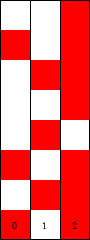
\includegraphics[width=.75\textwidth]{9/input.png}
		\caption{Input}
		\label{subfig:3neur_in}
	\end{subfigure}
	\hspace{1em}
	\begin{subfigure}{.3\textwidth}
		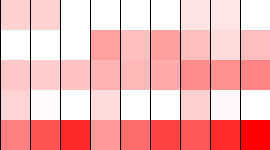
\includegraphics[width=\textwidth]{9/out0.png}
		\caption{Data after first transform}
	\end{subfigure}
	\hspace{1em}
	\begin{subfigure}{.3\textwidth}
		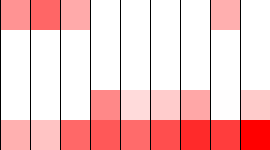
\includegraphics[width=\textwidth]{9/out1.png}
		\caption{Data after convolutional layer}
		\label{subfig:3neur_out1}
	\end{subfigure}
	\caption{Path of data through network, up to final transform}
	\label{fig:3neur_input}
\end{figure}

The last transformation of the network involves a matrix multiplication of the 
final layer weights\footnote{see appendix} with the data in 
\ref{subfig:3neur_out1}. This produces the adjacency matrix found in figure 
\ref{fig:3neur_pred}.

\begin{table}[h]
	\centering
	\begin{tabular}{l|lll}
		  & 0 	& 1   & 2\\
		\hline
		0 & .02 & .03 & .01\\
		1 & .99 & .01 & -.01\\
		2 & 1.00 & 1.00 & .02
	\end{tabular}
	\captionof{figure}{Output for input data in figure \ref{subfig:3neur_in}}
	\label{fig:3neur_pred}
\end{table}

\section{Applicability Beyond Training Data}
As described in \ref{subsubsec:hotswap}, the fact that our model is trained on 
data produced by only one generator is of little consequence; due to its 
structure, the only information it can learn is relational; i.e., 
per-neuron-pair. Consider the following examples, in which data was produced 
from several generator networks and fed into the model described in 
\ref{results_3neur}:


TODO: add examples of input and output data to 3.2.1 and 3.2.2.

\subsection{Inverted Network}
\begin{table}[h]
	\centering
	\begin{tikzpicture}[baseline=(current bounding box.center),->,>=stealth', 
	node distance=5em, semithick]
	\tikzstyle{every state}=[fill=none, draw=black, text=black]

		\node[state] (0) {0};
		\node[state] (1) [right of=0] {1};
		\node[state] (2) [below right of=0] {2};
	
		\path 	(2) edge node {} (1)
				(2) edge node {} (0)
				(1) edge node {} (0);
	\end{tikzpicture}
	\hspace{2em}
	\begin{tabular}{l|lll}
		  & 0 & 1 & 2\\
		\hline
		0 & 0 & 1 & 1\\
		1 & 0 & 0 & 1\\
		2 & 0 & 0 & 0
	\end{tabular}
	\captionof{figure}{Inverted version of figure \ref{fig:2simplex+adjacency}}
	\label{fig:2simplexVar1}
\end{table}
\noindent Despite being a complete inversion of the generator used to train the 
model in \ref{results_3neur}, reconstruction of this network is simple.

\begin{table}[h]
	\centering
	\begin{minipage}{.1\textwidth}
		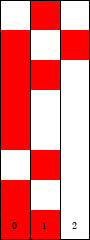
\includegraphics[width=\textwidth]{var1/input.png}
	\end{minipage}
	\hspace{2em}
	$\Rightarrow$
	\hspace{2em}
	\begin{tabular}{l|lll}
		  & 0 & 1 & 2\\
		\hline
		0 & .01 & 1.00 & 1.00\\
		1 & .01 & .02 & 1.00\\
		2 & 0 & .02 & .01
	\end{tabular}
\end{table}

\subsection{Cyclical Network}
\label{subsec:cyclical}
\begin{table}[h]
	\centering
	\begin{tikzpicture}[baseline=(current bounding box.center),->,>=stealth', 
	node distance=5em, semithick]
	\tikzstyle{every state}=[fill=none, draw=black, text=black]

		\node[state] (0) {0};
		\node[state] (1) [right of=0] {1};
		\node[state] (2) [below right of=0] {2};
	
		\path 	(2) edge node {} (1)
				(0) edge node {} (2)
				(1) edge node {} (0);
	\end{tikzpicture}
	\hspace{2em}
	\begin{tabular}{l|lll}
		  & 0 & 1 & 2\\
		\hline
		0 & 0 & 1 & 0\\
		1 & 0 & 0 & 1\\
		2 & 1 & 0 & 0
	\end{tabular}
	\captionof{figure}{Cyclical 3-neuron network}
	\label{fig:2simplexVar2}
\end{table}

\noindent For a cyclical network, the situation is not quite so simple. Due to 
the perpetual propagation of spikes through the generator, additional random 
spiking can cause the input data to become an impenetrable mess. Tempering the 
spike rate to 0.05 produces workable data, but the results are neither so clean 
nor
consistent as for terminating networks.  


